\documentclass[12pt]{amsart}
\usepackage[dvipdfmx]{graphicx}
\usepackage{amsmath,amssymb,amsthm,bm,wrapfig}
\theoremstyle{definiton}
\newtheorem{theorem}{定理}
\newtheorem*{lemma*}{補題}
\title{電子計算機及び実習２　最終課題}

\author{三森 誠真}

\begin{document}

\begin{abstract}
本論文では、Lebesgue積分論における重要な定理として, Lebesgueの収束定理について述べる.
\end{abstract}

\maketitle

\section{はじめに}
　基礎解析学2Aの授業で関数列について学んだ際, 極限と積分を交換できる定理について扱った.項別積分の性質はマクローリン展開やフーリエ級数といった解析学のあらゆる面に応用される大事なものであるが, 微分積分学の範囲では交換条件には関数列の一様収束性という強い仮定が必要だった.そこでLebesgue積分の概念を導入することにより関数列の一様収束性を必要とせずとも極限と積分の交換が可能となる定理の存在について知ったことが本論文を執筆するに至ったきっかけである.本論文ではLebesgueの収束定理の証明を目標とし, まずは準備として単調収束定理とFatouの補題について紹介し, またその証明について述べていきたい.

\bigskip

\section{準備}
この章では, Lebesgueの収束定理の証明の準備を行う.

\begin{theorem}
[単調収束定理, Monotone Convergence Theorem]
\end{theorem}
測度空間($X, \mathcal{F}, \mu$)から$\overline{\mathbb{R}}$への非負可測関数列$\{f_n\}$が
任意の$x \in X$に対して, $f_n(x) \le f_{n+1} (x)$, かつ
$\displaystyle \lim_{n \to \infty} f_n(x) = f(x)$ (各点収束) を満たすとする. このとき, 
$f$は非負可測関数であって, 

$\displaystyle \lim_{n \to \infty} \displaystyle \int_X f_n(x) d\mu$ =
$\displaystyle \int_X f(x) d\mu$ \ が成立する.

\bigskip

\begin{proof}
まず, 任意の$\lambda \in \mathbb{R}$に対して,

$\left\{x \middle| \displaystyle \limsup_{n \to \infty} f_n(x) > \lambda \right\}$ = 
$\displaystyle \bigcap_{n=1}^{\infty} \displaystyle \bigcup_{k=n}^{\infty}$
$\{x | f_k(x) > \lambda\} \in \mathcal{F}$, 

$\left\{x \middle| \displaystyle \liminf_{n \to \infty} f_n(x) > \lambda \right\}$ =
$\displaystyle \bigcup_{n=1}^{\infty} \displaystyle \bigcap_{k=n}^{\infty}$
$\{x | f_k(x) > \lambda\} \in \mathcal{F}$ \ が成り立つので, 

$\displaystyle \limsup_{n \to \infty} f_n$と$\displaystyle \liminf_{n \to \infty} f_n$が可測関数であることがわかり, よって$f$は可測関数.
そして, 積分の単調性より, $\displaystyle \int_X f_n(x) d\mu \le \displaystyle \int_X f(x) d\mu$
が言えるので, 
$\displaystyle \lim_{n \to \infty} \displaystyle \int_X f_n(x) d\mu \le$ $\displaystyle \int_X f(x) d\mu$ ───\textcircled{\scriptsize 1} が成立.


よって, 以下では逆向きの不等式を示していく.
まず, $0 \le \varphi \le f$ を満たすような可測単関数$\varphi$を
$\varphi(x) := \displaystyle \sum_{i=1}^N \alpha_i \chi_{E_i}(x)$ 
($\alpha_i > 0, E_i \in \mathcal{F})$ と定義し, さらにある集合$X_n$を任意の$c \in (0,1)$に対して
$X_n := \{x \in X | f_n(x) \ge c\varphi(x) \}$ と定義すると, $f_n$が可測関数であることより, $X_n$
\marginpar{\vbox to 0.88zw{\hbox to 50zw{\hss
    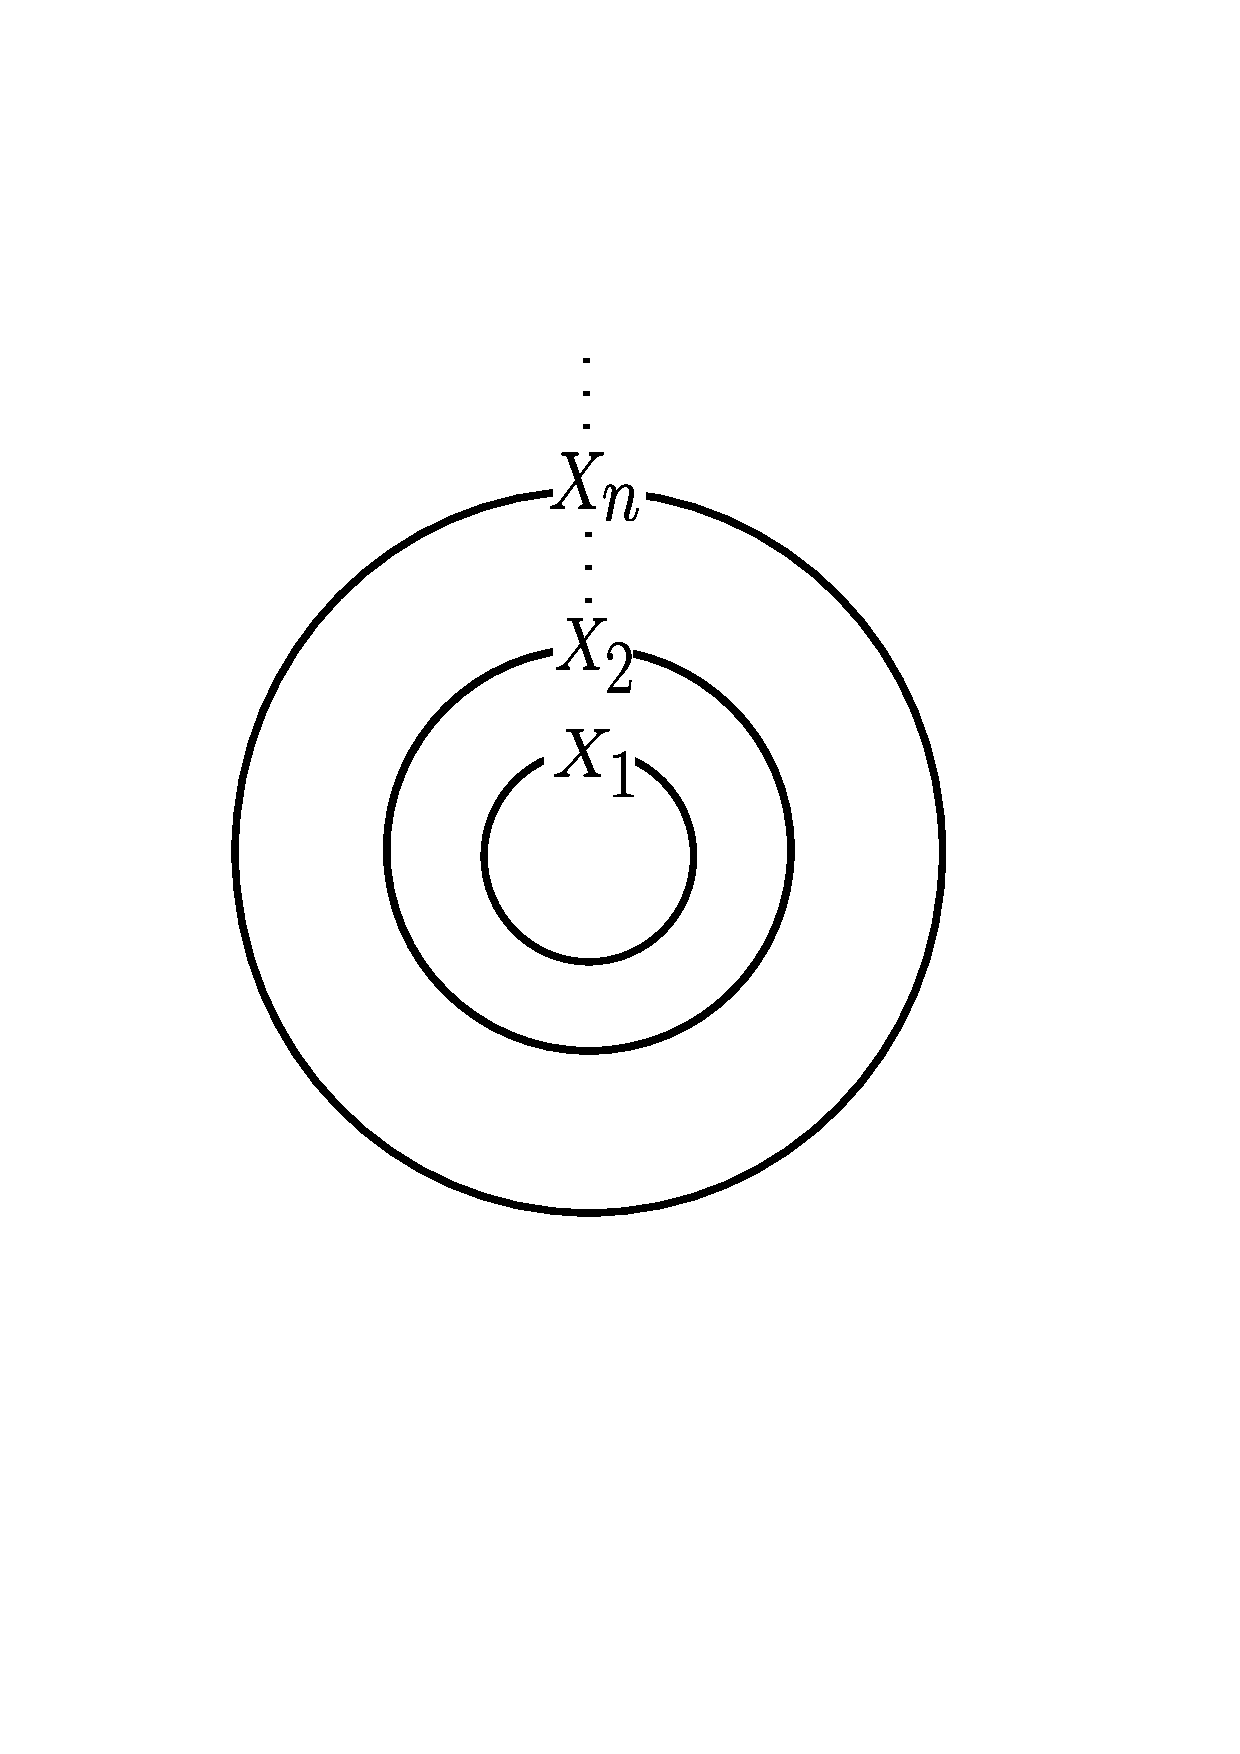
\includegraphics[height=13zw]{tanchozouka.pdf}}\vss}}
は可測集合. さらに, $X_n$は単調増加して $X = \displaystyle \bigcup_{n=1}^{\infty} X_n$ が成立する. このとき, $X_n \uparrow X$ より, $\mu(X_n) \uparrow \mu(X)$ なので,

$\displaystyle \lim_{n \to \infty} \displaystyle \int_{X_n} \varphi(x) d\mu$ =
$\displaystyle \lim_{n \to \infty} \displaystyle \sum_{i=1}^{N} \alpha_i\,\mu(E_i \cap X_n)$ =
$\displaystyle \sum_{i=1}^{N} \alpha_i\,\mu(E_i \cap X)$ =
$\displaystyle \int_{X} \varphi(x) d\mu$

\begin{align*}
\text{よって,} \ 
\displaystyle \lim_{n \to \infty} \displaystyle \int_X f_n(x) d\mu
&\ge \displaystyle \lim_{n \to \infty} \displaystyle \int_{X_n} f_n(x) d\mu \ \ \ (\because X_n \subset X) \\
&\ge c\displaystyle \lim_{n \to \infty} \displaystyle \int_{X_n} \varphi(x) d\mu \\
&= c\displaystyle \int_X \varphi(x) d\mu
\end{align*}

$c$は$0<c<1$の範囲で任意に取ってきているので,

$\displaystyle \lim_{n \to \infty} \displaystyle \int_X f_n(x) d\mu \ge$
$\displaystyle \int_X \varphi(x) d\mu$ \ が成立し,

$\displaystyle \int_X f(x) d\mu$ = 
$\sup \left\{\displaystyle \int_X \psi(x) d\mu \middle| \psi \text{は} 0 \le \psi \le f \text{を満たす単関数} \right\}$

なので, 
$\displaystyle \lim_{n \to \infty} \displaystyle \int_X f_n(x) d\mu \ge$
$\displaystyle \int_X f(x) d\mu$ ───\textcircled{\scriptsize 2}

したがって, \textcircled{\scriptsize 1}, \textcircled{\scriptsize 2}より
$\displaystyle \lim_{n \to \infty} \displaystyle \int_X f_n(x) d\mu$ = 
$\displaystyle \int_X f(x) d\mu$ \ が得られる.
\end{proof}

\section{主定理の証明}
本章では, Fatouの補題をもとにLebesgueの収束定理の証明を行う.

\begin{lemma*}[Fatouの補題, Fatou's lemma]
\end{lemma*}
測度空間($X, \mathcal{F}, \mu$)から$\overline{\mathbb{R}}$への可測関数列$\{f_n\}$が非負ならば, 

$\displaystyle \int_X \displaystyle \liminf_{n \to \infty} f_n(x) d\mu \le$
$\displaystyle \liminf_{n \to \infty} \displaystyle \int_X f_n(x) d\mu$ \ が成り立つ.

\bigskip

\begin{proof}
まず, 自然数$k$を任意にとる. このとき,  
$\displaystyle \inf_{n \ge k} f_n(x) := \inf \{f_n(x) | n \ge k \}$は可測関数であり, 任意の$j \ge k$に対して
$\displaystyle \inf_{n \ge k} f_n(x) \le f_j(x)$ なので, 
$\displaystyle \int_X \displaystyle \inf_{n \ge k} f_n(x) d\mu \le \displaystyle \int_X f_j(x) d\mu$
$ \le \displaystyle \inf_{j \ge k} \displaystyle \int_X f_j(x) d\mu$

この両辺を$k \to \infty$とすると, 
$\displaystyle \lim_{k \to \infty} \displaystyle \int_X \displaystyle \inf_{n \ge k} f_n(x) d\mu \le$
$\displaystyle \liminf_{k \to \infty} \displaystyle \int_X f_k(x) d\mu$
また, $\displaystyle \inf_{n \ge k} f_n(x)$は$k$に関して単調増加列となっているので, 単調収束定理から
$\displaystyle \lim_{k \to \infty} \displaystyle \int_X \displaystyle \inf_{n \ge k} f_n(x) d\mu$ = 
$\displaystyle \int_X \displaystyle \lim_{k \to \infty} \displaystyle \inf_{n \ge k} f_n(x) d\mu$ = 
$\displaystyle \int_X \displaystyle \liminf_{k \to \infty} f_k(x) d\mu$
$k$は任意の自然数なので, $\displaystyle \int_X \displaystyle \liminf_{n \to \infty} f_n(x) d\mu \le$
$\displaystyle \liminf_{n \to \infty} \displaystyle \int_X f_n(x) d\mu$ \ となることがこれで示された.
\end{proof}

\bigskip

\begin{theorem}[Lebesgueの収束定理, Lebesgue's Dominated Convergence Theorem]
\end{theorem}

測度空間($X, \mathcal{F}, \mu$)から$\overline{\mathbb{R}}$への可測関数列$\{f_n\}$が
任意の$x \in X$に対して, $\displaystyle \lim_{n \to \infty} f_n(x) = f(x)$ (各点収束)を満たし, 
$|f_n(x)| \le g(x)$ となるLebesgue可積分な関数$g$が存在するならば, 

 \ \ \ \ \ \ \ \ \ \ \ \ \ \ \ $\displaystyle \lim_{n \to \infty} \displaystyle \int_X f_n(x) d\mu$ =
$\displaystyle \int_X f(x) d\mu$ \ が成立する.

\bigskip

\begin{proof}
まず, $f_n, f, g$は$X$上でLebesgue可積分である.

$-g(x) \le f_n(x) \le g(x)$より, $g(x)-f(x) \ge 0$, 
$g(x) + f(x) \ge 0$ が得られるので, Fatouの補題より, 
\begin{align*}
\displaystyle \int_X g(x) d\mu - \displaystyle \int_X f(x) d\mu
= \displaystyle \int_X (g(x) - f(x)) d\mu
&= \displaystyle \int_X \displaystyle \liminf_{n \to \infty} (g(x) - f_n(x)) d\mu \\
&\le \displaystyle \liminf_{n \to \infty} \displaystyle \int_X (g(x) - f_n(x)) d\mu \\
&= \displaystyle \int_X g(x) d\mu - \displaystyle \limsup_{n \to \infty} \displaystyle \int_X f_n(x) d\mu
\end{align*}
よって, $\displaystyle \int_X f(x) d\mu \ge \displaystyle \limsup_{n \to \infty} \displaystyle \int_X f_n(x) d\mu$
───\textcircled{\scriptsize 1}

\begin{align*}
\displaystyle \int_X g(x) d\mu + \displaystyle \int_X f(x) d\mu
= \displaystyle \int_X (g(x) + f(x)) d\mu
&= \displaystyle \int_X \displaystyle \liminf_{n \to \infty} (g(x) + f_n(x)) d\mu \\
&\le \displaystyle \liminf_{n \to \infty} \displaystyle \int_X (g(x) + f_n(x)) d\mu \\
&= \displaystyle \int_X g(x) d\mu + \displaystyle \liminf_{n \to \infty} \displaystyle \int_X f_n(x) d\mu
\end{align*}
よって, $\displaystyle \int_X f(x) d\mu \le \displaystyle \liminf_{n \to \infty} \displaystyle \int_X f_n(x) d\mu$
───\textcircled{\scriptsize 2}

\textcircled{\scriptsize 1}, \textcircled{\scriptsize 2}より, 
$\displaystyle \lim_{n \to \infty} \displaystyle \int_X f_n(x) d\mu$ =
$\displaystyle \int_X f(x) d\mu$
\end{proof}

\bigskip

以上が主定理の証明となる. 最後に参考文献を挙げる.

\bigskip

\begin{thebibliography}{9}
\bibitem{Arai}
新井仁之, ルベーグ積分講義─ルベーグ積分と面積０の不思議な図形たち, 日本評論社 (2003)

\bibitem{Aikawa・Kobayashi}
相川弘明・小林政晴, ルベーグ積分　要点と演習, 共立出版 (2018)

\bibitem{Hara}
原啓介, 測度の考え方～測り測られることの数学～, 技術評論社 (2023)

\bibitem{Yoshida}
吉田洋一, ルベグ積分入門, ちくま学芸文庫 (2015)
\end{thebibliography}


\end{document}
